\chapter{Performance Analysis}
\label{chap:performance_analysis}

In this section, we present the results of our proposed acceleration techniques and detail the fitness function employed consistently across all experiments. The primary objective of the fitness function is to balance predictive performance with hardware efficiency, ensuring that the selected models are not only accurate but also suitable for deployment on resource-constrained devices.

As a baseline reference, we consider the unoptimized training setup consisting of 70 epochs. All subsequent optimization strategies aim to reduce the total training time while preserving the relative ranking of model performance. In particular, emphasis is placed on minimizing the risk of misranking high-performing models due to premature stopping or overly aggressive pruning. Maintaining ranking fidelity is crucial to ensure that acceleration techniques do not compromise the overall model selection process.

The fitness function is defined as:

\sloppy
\begin{equation}
\text{Fitness} =
\begin{cases}
\begin{aligned}
0.7 \cdot \text{Accuracy}_{\text{TFLite}} 
+ 0.2 \cdot \left(1 - \dfrac{\text{RAM}}{\text{MaxRAM}}\right) \\
+ 0.1 \cdot \left(1 - \dfrac{\text{Flash}}{\text{MaxFlash}}\right),
\end{aligned}
& \text{if } \text{RAM} \leq \text{MaxRAM} \land \text{Flash} \leq \text{MaxFlash} \\
-1000, & \text{otherwise}
\end{cases}
\label{eq:fitness_function}
\end{equation}



This formulation was chosen to explicitly incorporate hardware constraints into the optimization objective. Including this fitness function, we effectively guide the Genetic Algorithm (GA) to prioritize models that are not only accurate but also memory-efficient.

Notably, although the highest accuracy achieved during training (at 70 epochs) was approximately 60\%, the fitness function allows models with lower accuracy (e.g., around 40\%) to outperform others if they demonstrate significantly lower memory usage. However, by assigning a higher weight (0.7) to the accuracy term in the fitness function, we ensure that performance remains the primary objective. This is especially important considering that accuracy typically ranges from 0.3 to 0.65, while the normalized RAM and Flash components can span from 0 to 0.85. Without the weighted terms, the smallest models would consistently dominate the selection process—regardless of their predictive performance. The chosen weighting strategy ensures that the evolutionary search favors architectures that are not only compact and efficient but also sufficiently accurate for deployment.

It's important to note that microcontrollers are typically designed for specific tasks within embedded systems, combining processing, memory, and input/output peripherals on a single chip. This design makes them cost-effective and power-efficient for dedicated applications. In such scenarios, as long as the model fits within the available memory constraints of the microcontroller, such as the 256KB SRAM of the Arduino Nano 33 BLE Sense , the exact memory consumption becomes less critical. Therefore, the fitness function's weighting ensures a balance between model accuracy and resource efficiency, aligning with the practical considerations of deploying models on resource-constrained devices \cite{arduino_nano33ble}.

In this chapter, we review the results of the optimization algorithms discussed in Chapter~\ref{chap:nas_optimizations}. Many of these techniques aim to reduce the training time of the NAS algorithm while maintaining the integrity of model selection. To evaluate their effectiveness, we analyze both the percentage error in predictive performance and the total training time saved.

A key metric considered throughout this analysis is the mean squared error (MSE). In cases where an optimization misranks two models, we assess the severity of the misranking by comparing their fitness scores in the ground truth setting—defined by the full 70-epoch training. This provides a meaningful indication of the impact of prediction errors, helping us quantify how much the optimization distorts the model selection process.

The MSE for misranked pairs is computed as follows:

\begin{equation}
\text{MSE} = \frac{1}{N} \sum_{i=1}^{N} \left( \text{TrueFitness}_i - \text{TrueFitness}_j \right)^2
\end{equation}

where \( N \) is the total number of misranking errors, and \( \text{TrueFitness}_i \) and \( \text{TrueFitness}_j \) are the fitness scores of the misranked model pair \( (i, j) \) in the ground truth setup. A higher MSE indicates more severe misrankings, reflecting greater deviation from the ideal model selection.

Although the fitness function is normalized between 0 and 1 for consistency across experiments, it is important to consider the absolute performance range of the evaluated models. To provide additional context, we report the fitness scores of the best and worst models prior to normalization. This helps quantify the practical implications of misrankings by illustrating how much real-world performance (e.g., in terms of accuracy or hardware usage) separates the top-performing models from the least efficient ones.

\begin{table}[ht]
\centering
\caption{Fitness scores of best and worst models}
\begin{tabular}{lcc}
\toprule
Model & Raw Fitness Score & Description \\
\midrule
Best Model & 0.565 & High accuracy, low memory usage \\
Worst Model & 0.458 & Low accuracy, high memory \\
\bottomrule
\end{tabular}
\end{table}

To better interpret the severity of MSE values, we also compute the root mean squared error (RMSE) and express it relative to the raw fitness score range, i.e., \( \text{maxFitness} - \text{minFitness} = 0.107 \). This ratio indicates how large the average prediction error is in relation to the total performance spread among evaluated models:

\begin{equation}
\text{Relative RMSE} = \frac{\text{RMSE}}{0.565 - 0.458} = \frac{\text{RMSE}}{0.107}
\end{equation}

A small relative RMSE (e.g., under 15\%) implies that, even when misrankings occur, the models involved are very close in terms of real-world performance, suggesting minimal practical impact. Conversely, a large relative RMSE (e.g., above 40\%) indicates that the ranking errors involve models with substantially different fitness, potentially leading to significantly suboptimal deployment decisions. This contextualization allows us to bridge the gap between statistical misranking rates and their real-world consequences.




\section{Memory Estimation Experiment}
\label{sec:memory_estimation_experiment}
To assess the effectiveness of the proposed memory-aware optimization, a dedicated experiment was conducted in which the memory filtering mechanism was deliberately disabled. In this configuration, models exceeding the allowable RAM or flash memory constraints were not filtered out prior to training. Instead, any model violating the hardware limits was penalized post-training by assigning it a fixed fitness value of –1000. The purpose of this experiment was to investigate whether the genetic algorithm (GA) could inherently learn to avoid infeasible models, despite the lack of preemptive filtering.

Following a 4-hour NAS run, it became evident that only a limited number of models were successfully trained. This was primarily due to the fact that models with larger RAM and flash memory requirements consumed significantly more computational time—even for short training durations. In some cases, a single large model required up to four times the training time of a smaller, resource-efficient one (see Table~\ref{tab:taku_models}). This disparity in training time illustrates the inefficiency introduced by allowing oversized models to enter the search process.

Moreover, after evaluating all trained models, only a small fraction were found to be deployable on the Arduino Nano. While the RankNet-based predictor demonstrated some ability to identify promising architectures before training, its utility was limited in scenarios where the vast majority of candidates were infeasible. Specifically, when many models received the same penalty score (e.g., –1000), the RankNet network struggled to make meaningful comparisons during pairwise ranking. This led to stagnation in the learning process, as the predictor could not effectively differentiate between models based solely on invalid fitness values.

As illustrated in Figure~\ref{fig:memoryEstimationTest}, approximately \textbf{75\%} of the trained models were ultimately undeployable due to violating memory constraints. This result highlights the substantial inefficiencies introduced when memory-aware filtering is not applied. Beyond wasting training time on models that will later be discarded, the overall search process is slowed due to longer training cycles and increased difficulty in selecting promising candidates. Incorporating early memory estimation not only improves the efficiency of NAS by avoiding wasted computation, but also ensures that the evolutionary search is guided more effectively toward viable, deployable solutions.

\clearpage

\begin{table}[ht]
\noindent % removes indentation
\hspace*{-\oddsidemargin} % shift left based on page margin
\makebox[\linewidth][l]{%
\resizebox{1.20\textwidth}{!}{%
\begin{tabular}{|l|c|c|c|c|c|c|c|c|c|c|c|c|c|c|c|}
\hline
\textbf{Model} & \textbf{Train Acc} & \textbf{Test Acc} & \textbf{SWA Acc} & \textbf{TFLite Acc} & \textbf{Opt.} & \textbf{Precision} & \textbf{Recall} & \textbf{F1} & \textbf{RAM (KB)} & \textbf{Flash (KB)} & \textbf{TFLite (KB)} & \textbf{FLOPs} & \textbf{Fitness} & \textbf{Time (min)} & \textbf{Epochs} \\
\hline
TakuNet\_Init\_0 & 0.8922 & 0.5717 & 0.5717 & 0.5730 & adamw & 0.5712 & 0.5717 & 0.5690 & 546.91 & 15020.00 & 13731.02 & 31824133 & -1000.00 & 14.48 & 10 \\
TakuNet\_Mutant\_13 & 0.4719 & 0.4396 & 0.4396 & 0.4367 & adamw & 0.4342 & 0.4396 & 0.4304 & 52.18 & 316.71 & 321.56 & 750018 & 0.5130 & 4.92 & 10 \\
\hline
\end{tabular}
}}
\caption{Summary of two TakuNet models.}
\label{tab:taku_models}
\end{table}

\bigskip

\begin{figure}[ht]
    \centering
    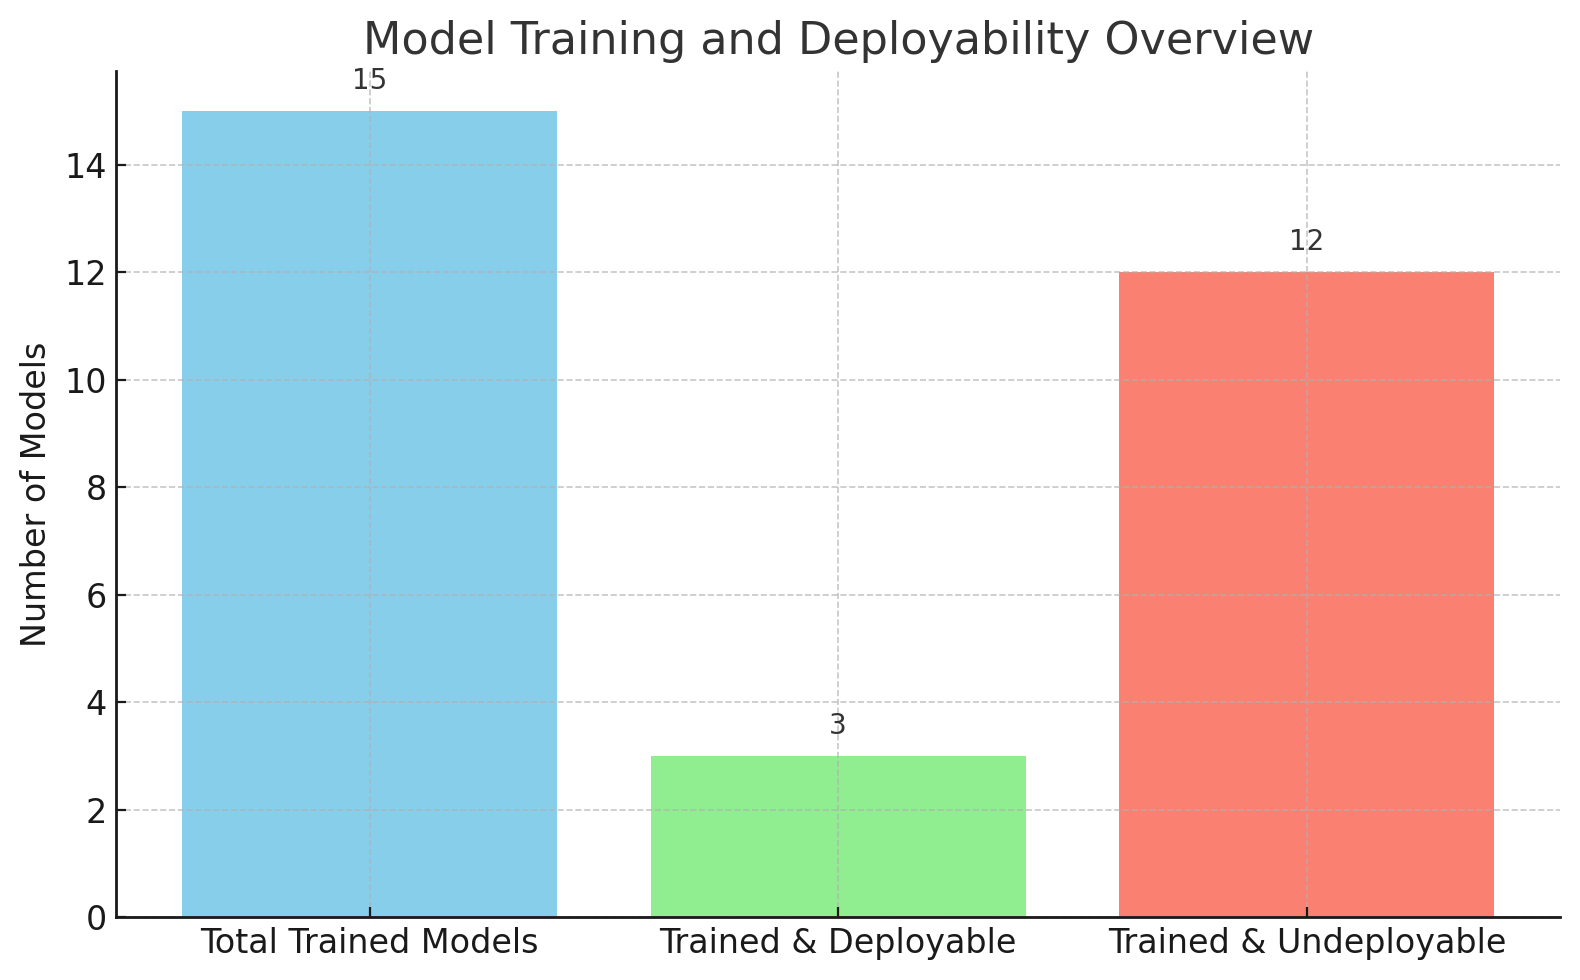
\includegraphics[width=0.85\linewidth]{Pictures/MemoryEstimationTest.png}
    \caption{MemoryEstimationTest}
    \label{fig:memoryEstimationTest}
\end{figure}





\section{RankNet Experiment}
\label{sec:ranknet_experiment}
In this experiment, we analyzed the outcomes of a large-scale NAS run that lasted approximately 10 hours. Given that our selection process is based on tournament comparisons, it is nearly impossible to recreate the exact pairwise matchups observed during the original run. To ensure transparency and reproducibility, we retained both the fitness scores and the parameter configurations of every model evaluated.

To evaluate the predictive performance of the RankNet model, we conducted \textbf{10{,}000 random pairwise comparisons} between different neural architectures, previously unseen to the RankNet. Our model was trained based on and initial population of \textbf{10 models} creating 45 pairs for training. In each comparison, the objective was to predict which of the two models would achieve superior performance. Given the randomness inherent in such pairings, a baseline model based on random guessing would be expected to achieve \textbf{50\% accuracy}. Despite this, \textbf{RankNet correctly identified the better-performing model in $\sim$85\% of the comparisons}, demonstrating strong predictive capability. Additionally, it achieved a mean squared error (MSE) of \textbf{1.15$\times$10\textsuperscript{-4}} on the \textit{normalized fitness function}, corresponding to a root mean squared error (RMSE) of \textbf{0.0107}. This translates to a \textbf{relative RMSE of 10.0\%}, indicating that even in cases where RankNet misranks two models, their actual performance is typically very close—thus limiting the potential negative impact of such errors (see Fig.~\ref{fig:RankNetComparison}).


\begin{figure}[ht]
    \centering
    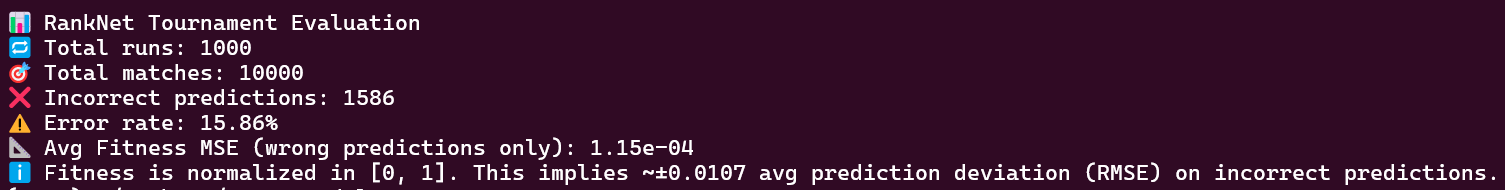
\includegraphics[width=1.05\linewidth]{Pictures/RankNetComparison.png}
    \caption{RankNet Comparison}
    \label{fig:RankNetComparison}
\end{figure}


These results highlight the strong predictive capability of the RankNet model. Achieving an $\sim$85\% accuracy in pairwise comparisons represents a substantial improvement over the 50\% accuracy expected from random guessing. In ranking tasks, such a margin is considered highly significant, especially when coupled with a very low mean squared error. Even relatively small improvements above chance can yield meaningful benefits in optimization scenarios \cite{freund1999large}, making this level of performance particularly impaction.

Moreover, in our NAS algorithm, RankNet's potential misjudgments are inherently mitigated. Specifically, we rely on RankNet's predictions only when neither of the competing models has been trained yet. This strategic usage ensures that the actual impact of any prediction error is reduced, and the overall effectiveness of the NAS procedure remains robust—even more so than what is reflected in this isolated evaluation.

While it is difficult to precisely quantify the overall speedup gained by integrating RankNet into the NAS process, the fact that it performs better than random guessing is already valuable. By more accurately identifying promising architectures early on, RankNet helps to avoid the training of clearly suboptimal models. This selective approach evidently contributes to reducing the total time and computational cost required by the NAS algorithm.


\section{Early Stoppage Experiment}

In this experiment, building upon previous observations, we aimed to stop the training of specific models early in order to reduce computational cost when it was likely that their final performance would be suboptimal. As previously discussed, the first few epochs of training tend to be the most informative. If a model fails to reach a predefined validation accuracy threshold by a given cutoff epoch, it is unlikely to outperform others later on. To exploit this, we designed a threshold-based early stopping strategy: during training, if the validation accuracy at a predefined cutoff epoch does not surpass a certain threshold, the training is terminated early. This approach simulates an informed pruning of under-performing models.

To evaluate the effectiveness of this method, we performed a grid search over various cutoff epochs and validation accuracy thresholds. For each configuration, we computed the estimated fitness using a normalized function that incorporates accuracy, RAM usage, and flash memory requirements (see Equation~\ref{eq:fitness_function}). We then used a tournament-style comparison to evaluate how closely these early estimates matched the final results of fully trained models. The configurations were assessed based on their prediction error rate and the total training time saved.

As shown in Table~\ref{tab:early_stopping_results}, the best configuration with an error rate below 19\% achieved a training time reduction of up to 19.48\%. This demonstrates that a well-calibrated threshold-based early stopping strategy can substantially reduce training costs with minimal impact on model selection accuracy.

It is important to note that, during the grid search, we deliberately restricted the range of both cutoff epochs and validation accuracy thresholds to cases where the validation accuracy exceeded 25\%. This constraint was applied to minimize noise in the comparisons, as models performing significantly below this level tended to produce unstable and uninformative results in the tournament-based evaluation. Furthermore, we found that similar optimal ranges of cutoff epochs and thresholds consistently appeared across multiple independent training runs and over different time periods. This recurring pattern reinforces the validity of our approach and supports the assumption that early validation performance serves as a reliable proxy for final model quality.


\begin{table}[ht]
\centering
\begin{tabular}{cccccc}
\toprule
Cutoff Epoch & Threshold & Error Rate (\%) & MSE & Time Saved (min) & Time Saved (\%) \\
\midrule
10  & 0.33 & 18.99 & 7.15e-04 & 108.35 & 19.48 \\
11  & 0.33 & 14.71 & 7.65e-04 & 105.51 & 15.28 \\
\vdots & \vdots & \vdots & \vdots & \vdots & \vdots \\
\bottomrule
\end{tabular}
\caption{Top 2 early stopping configurations ranked by time saved.}
\label{tab:early_stopping_results}
\end{table}




\section{Performance Stop Experiment}

In this experiment, we conducted a full 10-hour training run \textbf{without} applying the performance stop optimization described in Section~\ref{sec:performance_stop}.

Figure~\ref{fig:performanceStop} illustrates the proportion of models that could have been early-stopped, along with their corresponding projected loss in validation accuracy. This loss is calculated relative to the highest validation accuracy achieved by any model across all training experiments, thus providing a consistent global benchmark.

As depicted in the figure, approximately 10\% of the models incurred less than a 5\% loss in validation accuracy compared to the best-performing model. Moreover, 30\% and 55\% of the models stayed within 10\% and 20\% of the best, respectively. Remarkably, 90\% of the models remained within a 30\% margin, demonstrating that the majority of early-stopped models still maintained competitive performance.

To evaluate the efficiency gains of this approach, we applied a performance-based early stopping strategy across all discovered models. Assuming uniform epoch duration the un-optimized version required \textbf{556.10 minutes} of training. When Performance optimization was activated, a total of \textbf{214.57 minutes} of training time was saved, reducing the total compute time from \textbf{556.10 minutes} to \textbf{341.53 minutes}—a \textbf{38.59\%} reduction.

To assess the trade-off in decision quality, we conducted \textbf{10,000 random pairwise comparisons} between model candidates using both full and early-stopped fitness evaluations. As shown in Table~\ref{tab:performance_stopping_summary}, the early-stopped models resulted in a decision error rate of \textbf{22.00\%}, indicating that in the majority of cases, early termination preserved correct model ranking. Additionally, the mean squared error (MSE) between full and early-stopped validation accuracies was \textbf{4.36$\times$10\textsuperscript{-4}}, corresponding to a root mean squared error (RMSE) of \textbf{2.09$\times$10\textsuperscript{-2}}, which is approximately \textbf{$\approx 19.53\%$} relative to the observed range in validation accuracy. This suggests that, even when discrepancies occur, they are typically minor in practical terms.

\begin{table}[ht]
\centering
\begin{tabular}{ll}
\toprule
\textbf{Parameter} & \textbf{Value} \\
\midrule
No Change Patience & 10 \\
$\alpha$ (Window Size \%) & 0.30 (Epoch Diminishing Return: 21.0) \\
$\epsilon$ (Min Relative Improvement) & 0.07 \\
Error Rate & 22.00\% \\
RMSE & 2.09$\times$10\textsuperscript{-2} \\
MSE & 4.36$\times$10\textsuperscript{-4} \\
Original Training Time & 556.10 minutes ($\approx$9h 16m) \\
Training Time with Early Stopping & 341.53 minutes ($\approx$5h 41m) \\
Time Saved & 214.57 minutes \\
Percentage Time Saved & 38.59\% \\
\bottomrule
\end{tabular}
\caption{Performance-based early stopping summary}
\label{tab:performance_stopping_summary}
\end{table}

These findings support the effectiveness of performance-based early stopping in significantly reducing computational time while preserving acceptable accuracy. In practice, tolerating small projected performance losses can greatly enhance scalability and responsiveness in large-scale evolutionary or model selection tasks.


\begin{figure}[ht]
    \centering
    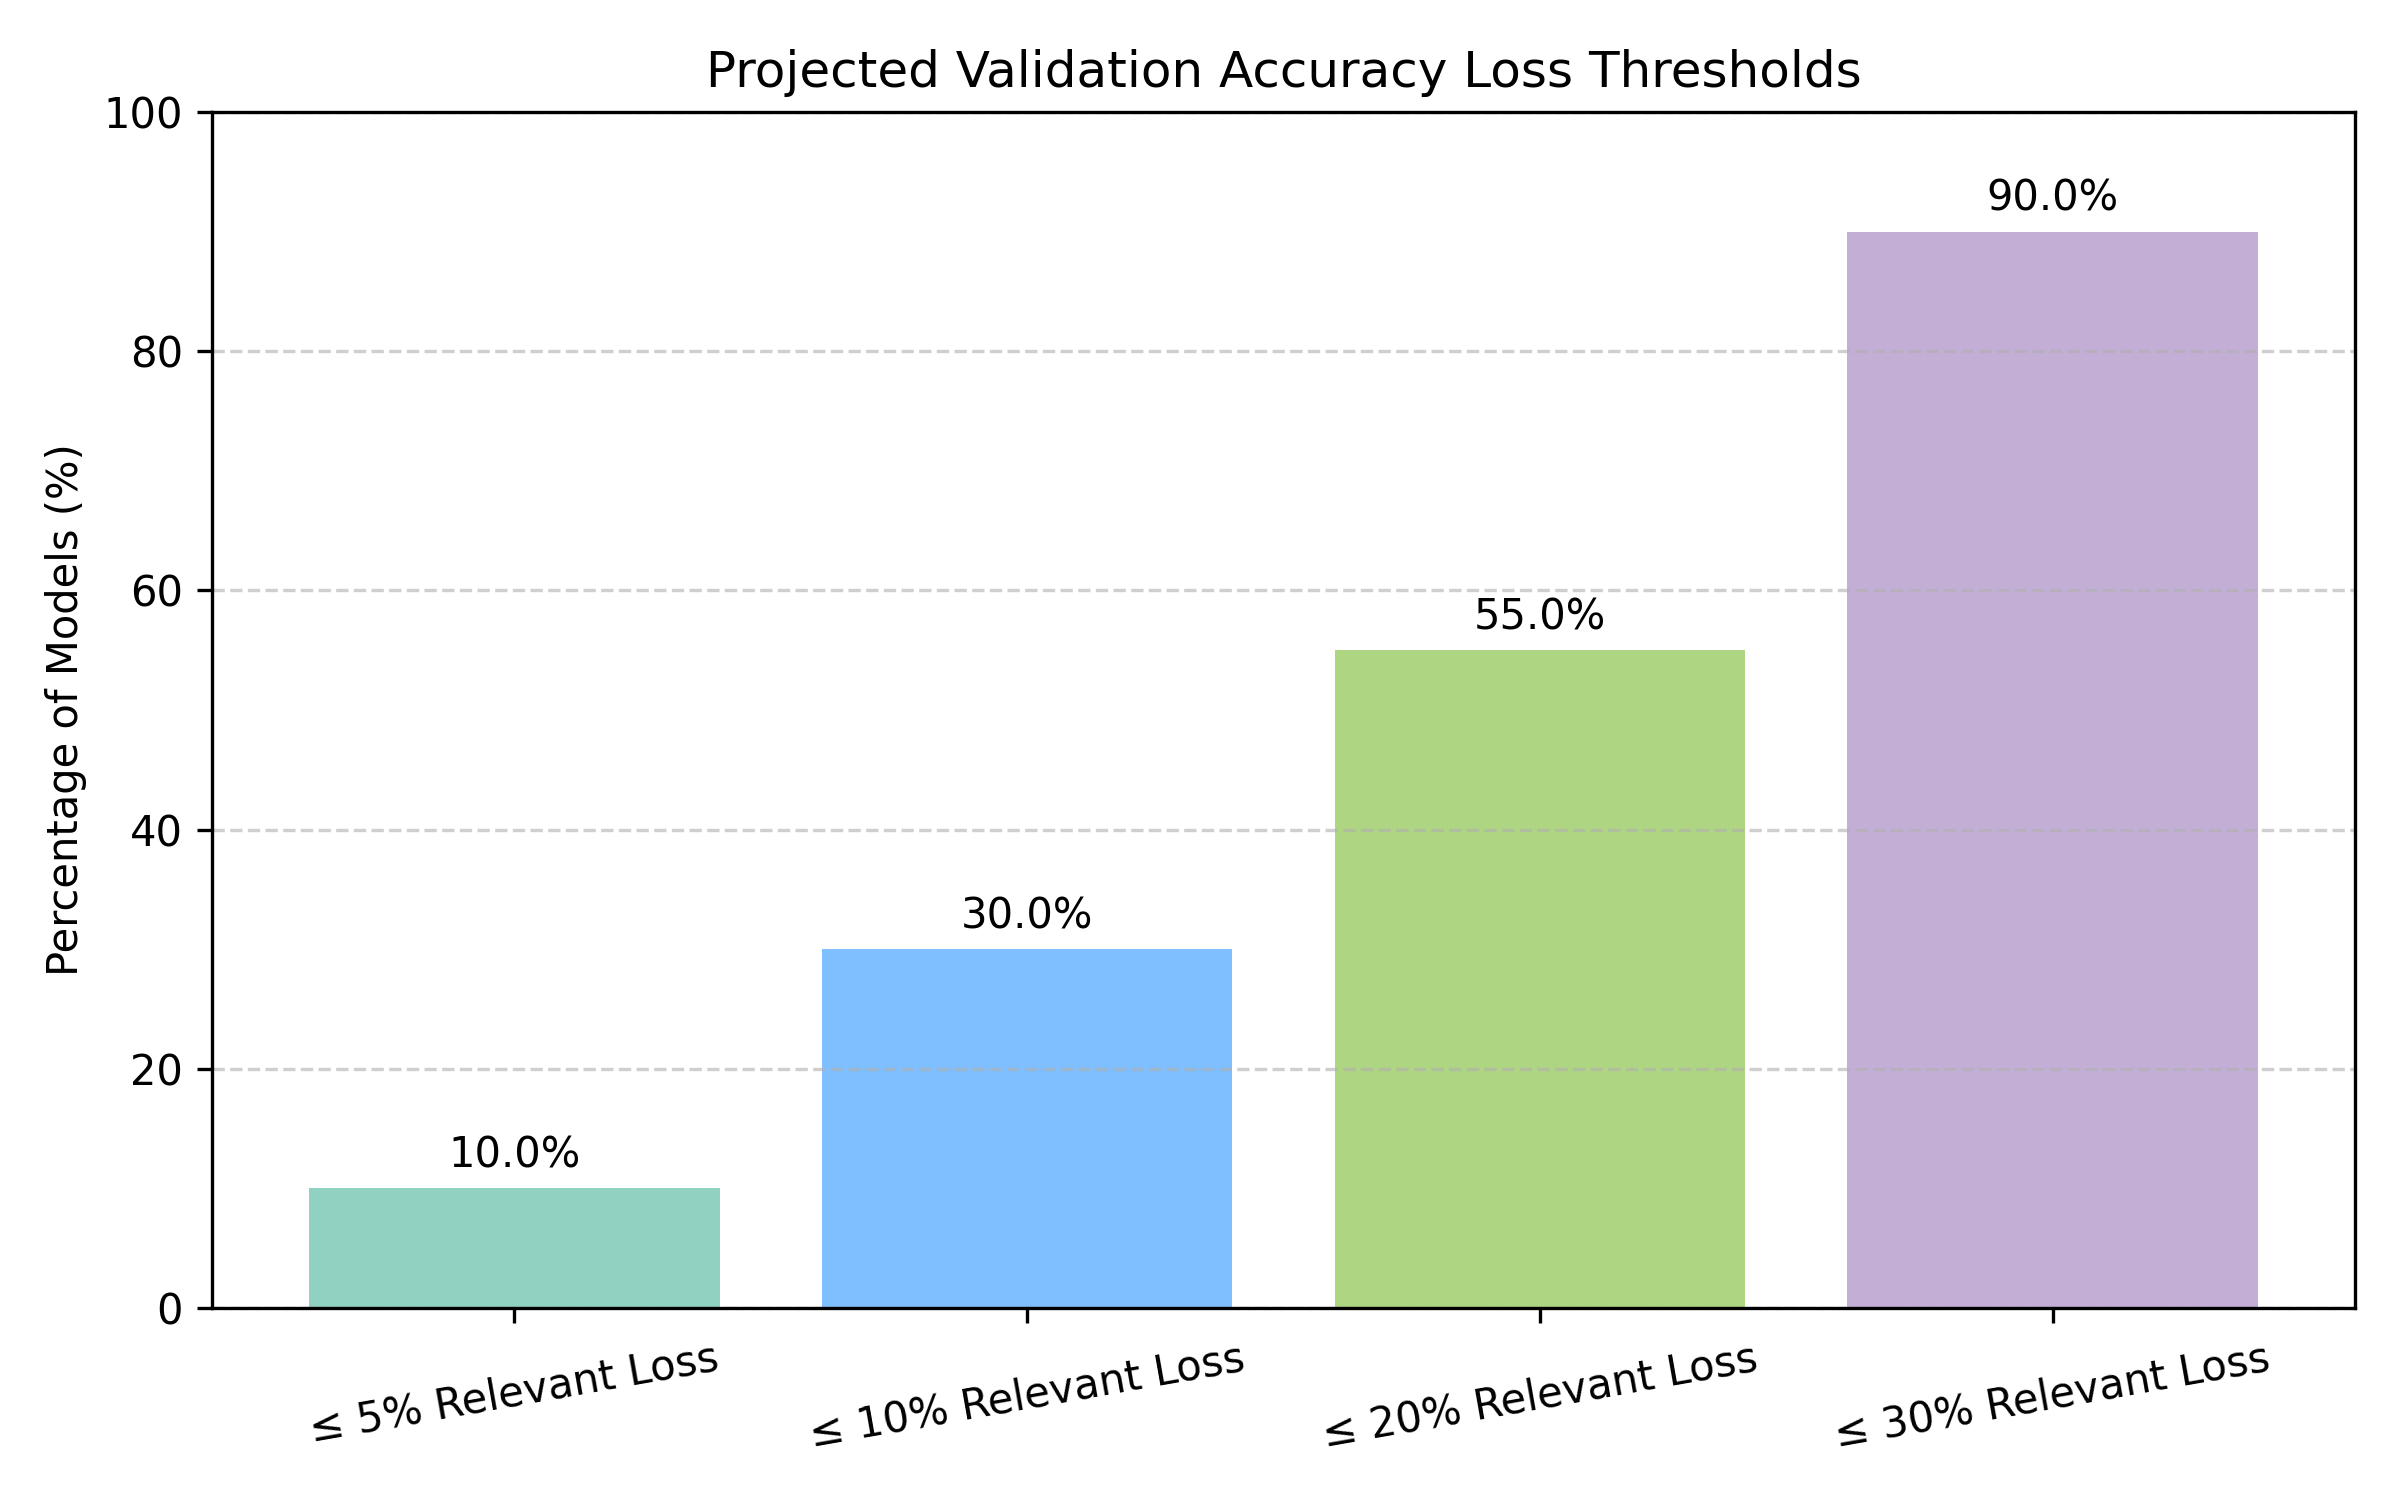
\includegraphics[width=0.85\linewidth]{Pictures/val_accuracy_loss_percentages.png}
    \caption{Percentage of models falling under various thresholds of projected validation accuracy loss relative to the best observed model.}
    \label{fig:performanceStop}
\end{figure}


\clearpage

\section{Learning Rate Experiment}

As previously discussed, cosine learning rate decay is theoretically expected to converge faster than traditional schedules such as \textbf{Step Decay}, \textbf{Constant Learning Rate}, or \textbf{Linear Decay} \cite{li2019exponential}  \cite{kim2021automated}. The motivation behind this experiment is to investigate whether we can achieve reliable performance predictions with fewer than the 70 training epochs we currently use as a baseline.

To test this hypothesis, we selected a set of models that were originally trained for 70 epochs. These models were then \textit{re-trained from scratch} using the cosine decay schedule but with \textbf{reduced epoch budgets}: specifically 10, 20, 30, and 50 epochs. For each of these training durations, we performed \textbf{10,000 random pairwise comparisons} to assess whether early-stopped models could still accurately reflect performance rankings.


\begin{table}[ht]
\centering
\begin{tabular}{|c|c|c|p{6cm}|}
\hline
\textbf{Epochs} & \textbf{Prediction Mistake} & \textbf{Avg. Time Reduction} & \textbf{Notes} \\
\hline
10 & $\sim$30\% & $\sim$85.24\% & Fastest training, but leads to high prediction errors and noisy rankings due to underfitting. \\
20 & $\sim$21\% & $\sim$62.12\% & Noticeable improvement in prediction stability; still some inconsistency, but a clear step up from 10 epochs. \\
30 & $\sim$16\% & $\sim$55\% & Achieves competitive accuracy, close to longer trainings; a strong compromise between performance and efficiency. \\
50 & $\sim$15\% & $\sim$32.69\% & Very stable predictions with minimal mistakes; however, the time savings are significantly reduced. \\
\hline
\end{tabular}
\caption{Comparison of RankNet pairwise accuracy using different training durations with cosine decay}
\label{tab:cosine_decay_results}
\end{table}


As shown in Table~\ref{tab:cosine_decay_results}, training for only \textbf{10 epochs} achieves the greatest average time reduction—over 85\%—but this comes with a high prediction mistake rate of approximately 30\%. This suggests that such a short training duration leads to significant underfitting, resulting in unstable and unreliable performance rankings.

At the other extreme, training for \textbf{50 epochs} yields the most accurate and stable predictions, with only ~15\% mistakes, closely approaching the reliability of the full 70-epoch baseline. However, the time savings at this level are considerably diminished—only around 32%—making it a less attractive option when computational efficiency is critical.

The intermediate settings of \textbf{20} and \textbf{30 epochs} stand out as promising trade-offs. Training for 20 epochs reduces time by more than 60\%, while cutting prediction mistakes to ~21\%, a notable improvement over the 10-epoch case. Meanwhile, 30 epochs further reduces mistakes to ~16\%, while still preserving over 50\% time savings. This suggests that models trained for 30 epochs achieve nearly the same predictive quality as the 50-epoch variant, but with better computational efficiency.

\textbf{In summary, training for 20 or 30 epochs appears to offer the most effective balance between prediction reliability and efficiency.} The choice between the two can be guided by specific application needs—whether prioritizing speed (20 epochs) or slightly higher accuracy (30 epochs).

These findings confirm that while cosine decay facilitates faster convergence compared to traditional learning rate schedules, a minimum training threshold remains essential for learning meaningful representations. Importantly, this also highlights the potential of cosine-based scheduling to accelerate neural architecture search (NAS) workflows by \textbf{reducing evaluation costs} without severely compromising the quality of performance ranking.


\section{Final Combined Optimization Experiment}

To evaluate the cumulative impact of the proposed optimization techniques, we conducted a final Neural Architecture Search (NAS) run in which all strategies were applied simultaneously. These included:

\begin{itemize}
    \item \textbf{Memory-Aware Filtering:} Prevents training of models that exceed microcontroller RAM and Flash constraints.
    \item \textbf{Cosine Learning Rate Decay:} Enables faster convergence, allowing models to reach informative performance with fewer epochs.
    \item \textbf{Performance-Based Early Stopping:} Halts training of underperforming models early to save computation time.
    \item \textbf{RankNet Selection:} Prioritizes promising models for evaluation based on predicted relative performance.
\end{itemize}


Among the applied strategies, two optimizations operate primarily outside the training loop: \textbf{Memory-Aware Filtering} and \textbf{RankNet Selection}. These techniques focus on reducing unnecessary training by identifying unpromising or infeasible models before any computational resources are spent on them.

\textbf{Memory-Aware Filtering} plays a crucial role in enforcing hardware constraints from the outset. By preemptively discarding models that exceed the microcontroller's RAM and Flash memory limits, the NAS process avoids wasting time on training architectures that are ultimately undeployable. As demonstrated in Section~\ref{sec:memory_estimation_experiment}, this significantly improves the throughput of the search and ensures that the computational effort is directed only toward viable candidates.

\textbf{RankNet Selection}, on the other hand, enables performance estimation without actual training. It leverages a learned surrogate model to predict relative performance among untrained architectures. This allows the NAS algorithm to prioritize which models are worth training, based on predicted pairwise comparisons. As discussed in Section~\ref{sec:ranknet_experiment}, even moderate prediction accuracy from RankNet translates into substantial time savings by preventing the evaluation of clearly suboptimal designs. Together, these external mechanisms form a powerful front-line filter that enhances both the scalability and efficiency of the NAS process.

It is important to distinguish between optimization techniques that operate independently of one another and those whose interactions must be carefully evaluated. 

The \textbf{external strategies}, namely \textbf{Memory-Aware Filtering} and \textbf{RankNet Selection}, are inherently orthogonal to the training process and can be safely applied in any setting. These techniques focus on early elimination of infeasible or unpromising architectures before training even begins, and therefore do not interfere with the dynamics of the training process itself.

In contrast, the \textbf{training-level optimizations}—specifically \textbf{Cosine Learning Rate Decay},\textbf{Performance-Based Early Stopping} and \textbf{Early Stoppage}—directly affect the way individual models are trained and evaluated. As such, their interaction must be empirically validated to ensure they work well in tandem. For example, while early stopping provides substantial speedup, its effectiveness depends heavily on the training length and convergence behavior introduced by the learning rate schedule.

\begin{comment}

Initially we decide to keep our Learning Rate Optimization at 20 epochs, are perviously discussed, this optimization achieved a 21\% error rate but also a 62.12\% speed up. Now when we added ( + ) the performance stop on top of it what we figure out is that that the error rate increase slightly at 24\% while it speed up the previous time 2.82\% -> 63.19\% from the initial starting training time. Then we applied the early stoppage optimization, in that we manage to see the error rate rise to 25\% but getting a crazy 85\%  -> 94.32\% speedup, while there was the possibility to achieve a 22\% error rate with a 4\% speedup -> 63.64\% with the early stoppage as well.



On the other hand starting from the training set to 30 epochs, we initially had an error rate 16\% and a speedup of 55\% . By appling in this the performance stoppage optimization we saw the error rate barely exceeding the 17\% , which makes sense as the slower the training , the more presice the upadtes, and the speedup gain was 18\% -> 62.66\% from the starting training time. On the other hand appling the early stoppage in this case gave the saem error rate as before (16.9 \%) but with only 3\% increase -> 55.83\%


Our findings indicate that \textbf{applying performance-based early stopping to 30-epoch cosine-trained models yields the most efficient and accurate configuration}. In this setting, models converge sufficiently for the early stopping criteria to make reliable decisions. Conversely, applying early stopping to shorter runs—such as 20 epochs—often led to premature termination of models that might have otherwise reached competitive performance. This suggests that performance-based stopping should be used selectively, only when the base training duration provides enough time for meaningful learning curves to emerge.
\end{comment}


To evaluate the impact of combining various optimization strategies, we conducted experiments starting from two different baseline training durations: 20 epochs and 30 epochs. In each case, we progressively applied three types of optimizations:
\begin{itemize}
    \item \textbf{Learning Rate Optimization (LR Opt.)}
    \item \textbf{Performance-Based Early Termination (Perf. Stop)}
    \item \textbf{Threshold-Based Early Stoppage (Early Stop)}
\end{itemize}

Table~\ref{tab:combined_optimizations} summarizes the error rates and the corresponding training speedup at each stage for both baseline configurations.

\begin{table}[h!]
\centering
\begin{tabular}{|p{4.5cm}|c|c|c|c|}
\hline
\textbf{Optimization Strategy} & \textbf{Error Rate (\%)} & \textbf{Average MSE} & \textbf{Speedup (\%)} & \textbf{Baseline epochs} \\ \hline
Learning Rate Optimization (LR Opt.)         & 21.00  & 7.61e-04 & 62.12 & 20 epochs \\ \hline
+ Performance Stop                           & 26.00 & 3.23e-04 & 63.19 & 20 epochs \\ \hline
+ Early Stoppage (Max)                       & 25.00 & 1.44e-04  & 85.00 & 20 epochs \\ \hline
+ Early Stoppage (Safe)                      & 22.00 & 2.14e-04  & 63.64 & 20 epochs \\ \hline
\hline
Learning Rate Optimization (LR Opt.)         & 16.00 & 7.63e-04 & 55.00 & 30 epochs \\ \hline
+ Performance Stop                           & 17.00 & 2.32e-04 & 64.66 & 30 epochs \\ \hline
+ Early Stoppage                             & 17.50 & 1.45e-04  & 59.83 & 30 epochs \\ \hline
\end{tabular}
\caption{Combined Optimization Effects at 20 and 30 Epoch Baselines}
\label{tab:combined_optimizations}
\end{table}


\subsection*{Discussion}

For the 20-epoch baseline, applying the learning rate optimization alone already provided a significant speedup of over 62\% with a moderate error rate of 21\%. Adding the performance-based stopping method slightly increased the error to 24\%, but resulted in a small gain in speedup, pushing it to 63.19\%.

The inclusion of early stoppage further amplified the benefits. In the most aggressive configuration, the error rose to 25\% but with an outstanding speedup of over 85\%. Alternatively, a safer threshold setting achieved 22\% error with a 63.64\% speedup—balancing performance and computational savings effectively.

For the 30-epoch baseline, the learning rate optimization alone achieved a strong 55\% speedup with a low 16\% error. Adding the performance stop mechanism led to a negligible increase in error (17.1\%) while improving the overall speedup to 62.66\%. Finally, applying early stoppage resulted in almost no additional error (16.9\%) and a minor speedup increase to 55.83\%.

\subsection*{Insights}

These results suggest that:
\begin{itemize}
    \item \textbf{Early stoppage offers dramatic computational savings} when error tolerance is flexible.
    \item \textbf{Performance-based stopping provides consistent, moderate improvements} in both speed and accuracy filtering.
    \item \textbf{The effectiveness of each method depends on the baseline epoch length}—aggressive methods yield larger gains when the starting budget is smaller (e.g., 20 epochs).
    \item \textbf{Safer early stoppage thresholds can match performance with minimal sacrifice} in accuracy, making them highly practical.
\end{itemize}


\subsection{Final Comparison}

Taking into account the previous experimental results, it remains unclear which individual optimization provides the best overall performance within a fixed time budget. Among the two most dominant techniques, one consistently yields models with lower prediction error, while the other significantly accelerates the search process. This trade-off between accuracy and speed introduces ambiguity when trying to identify the most promising approach.

To address this, we conduct a comparative experiment where the NAS algorithm is executed independently using each optimized variant. For each run, we collect the set of non-dominated solutions—i.e., the Pareto front—representing the best trade-offs between competing objectives such as model accuracy, memory usage, and inference time. By analyzing and comparing these Pareto-optimal models across techniques, we aim to determine which optimization strategy consistently leads to superior results under resource and time constraints.

It is important to note that small variations in outcomes are expected, even when training the same model multiple times with identical data. These deviations can stem from inherent randomness in training procedures (e.g., weight initialization, mini-batch sampling) and should be considered within the bounds of scientific or statistical error. Therefore, our analysis focuses on meaningful performance trends rather than minor fluctuation